\label{Toplevel}

Nachdem der genaue Programmablauf niedergeschrieben war, konnten durch die Zeichnung eines Top-Level-Diagramms, alle Ein- und Ausgänge am Arduino definiert werden. \\
Durch die drei Taster Up Button, Enter Button und Sleep Button, sollte die Bedienung des Menüs ermöglicht werden. Der CO$_2$-Value in Abbildung \ref{fig:Toplevel} steht für den, vom Sensor gemessenen Wert, welcher abgespeichert und ausgegeben wird. \\
Wegen der anfangs definierten Anforderung, die gemessenen CO$_2$-Werte in einer CSV-kompatiblen Datei auf einer SD-Karte abzuspeichern, muss die Hardware einen Ausgang für die Text-Datei besitzen. Zudem benötigt diese einen weiteren Port für die Ausgabe am \ac{LCD}-Display und vier weitere für die drei \ac{LED}s zur Interpretation der Luftgüte und die, zur Simulation des Fensterscheibenmotors. \\

\begin{figure}[!hbt]
	\centering
	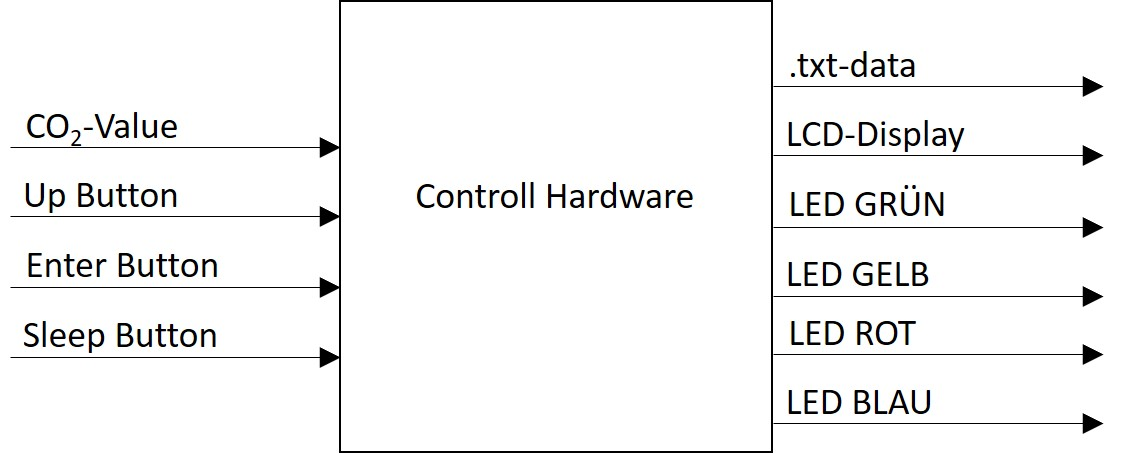
\includegraphics[width=0.7\linewidth]{Images/Topleveldiagramm}
	\caption{Entwurf der Top-Level-Architektur}
	\label{fig:Toplevel}
\end{figure}

\newpage